\documentclass[aspectratio=169,10pt]{beamer}
\usepackage[spanish,es-minimal,es-nodecimaldot]{babel}
\usepackage{booktabs,graphicx}
\usetheme{Oxygen}
\setbeamersize{text margin left=5mm,text margin right=5mm}
\setbeamerfont{frametitle}{size=\large,series=\bfseries}
\setbeamertemplate{navigation symbols}{}
\graphicspath{{../figuras/}{documentos/figuras/}}
\newcommand{\autores}{Sebastián Mindiola \and William Andres Velasquez Ruiz \and Jhon Eduardo Meneses Viecco}

\title[Rendimiento agrícola en el Cesar]{Rendimiento agrícola en el Cesar}
\subtitle{Evaluaciones Agropecuarias Municipales, 2007--2018}
\author[Equipo EVA Cesar]{\autores}
\institute[UNAL]{Universidad Nacional de Colombia\\
Programación en Lenguajes Estadísticos (2026-2) · Docente Yoselin Nieto G.}
\date[2026]{2026}

\begin{document}

{
\addtobeamertemplate{headline}{\vspace*{-0.5cm}}{}
\begin{frame}
  \titlepage
\end{frame}
}

\begin{frame}{Así llegan los datos de EVA}
\small
\texttt{head()} del subconjunto del Cesar, tras leer las cantidades del CSV.
Las cinco filas corresponden a aguacate.
\vspace{.6em}

\centering
\begin{tabular}{lrrrrr}
\toprule
Municipio & Periodo & Sembrada (ha) & Cosechada (ha) & Producción (t) & Rend. (t/ha)\\
\midrule
Valledupar          & 2007 & 713 & 713 & 5.704 & 8,00\\
La Jagua de Ibirico & 2007 & 430 & 430 & 2.150 & 5,00\\
La Paz              & 2007 & 300 & 300 & 3.000 & 10,00\\
Pueblo Bello        & 2007 & 105 & 103 & 830 & 8,06\\
San Martín          & 2007 & 90 & 80 & 640 & 8,00\\
\bottomrule
\end{tabular}

\vspace{.8em}
En San Martín se cosecharon 80 de las 90 ha sembradas. El rendimiento es \(640/80=8\) t/ha.
\end{frame}


\begin{frame}{Distribución de los registros del Cesar}
\begin{columns}[c,totalwidth=\textwidth]
\column{.57\textwidth}
\centering
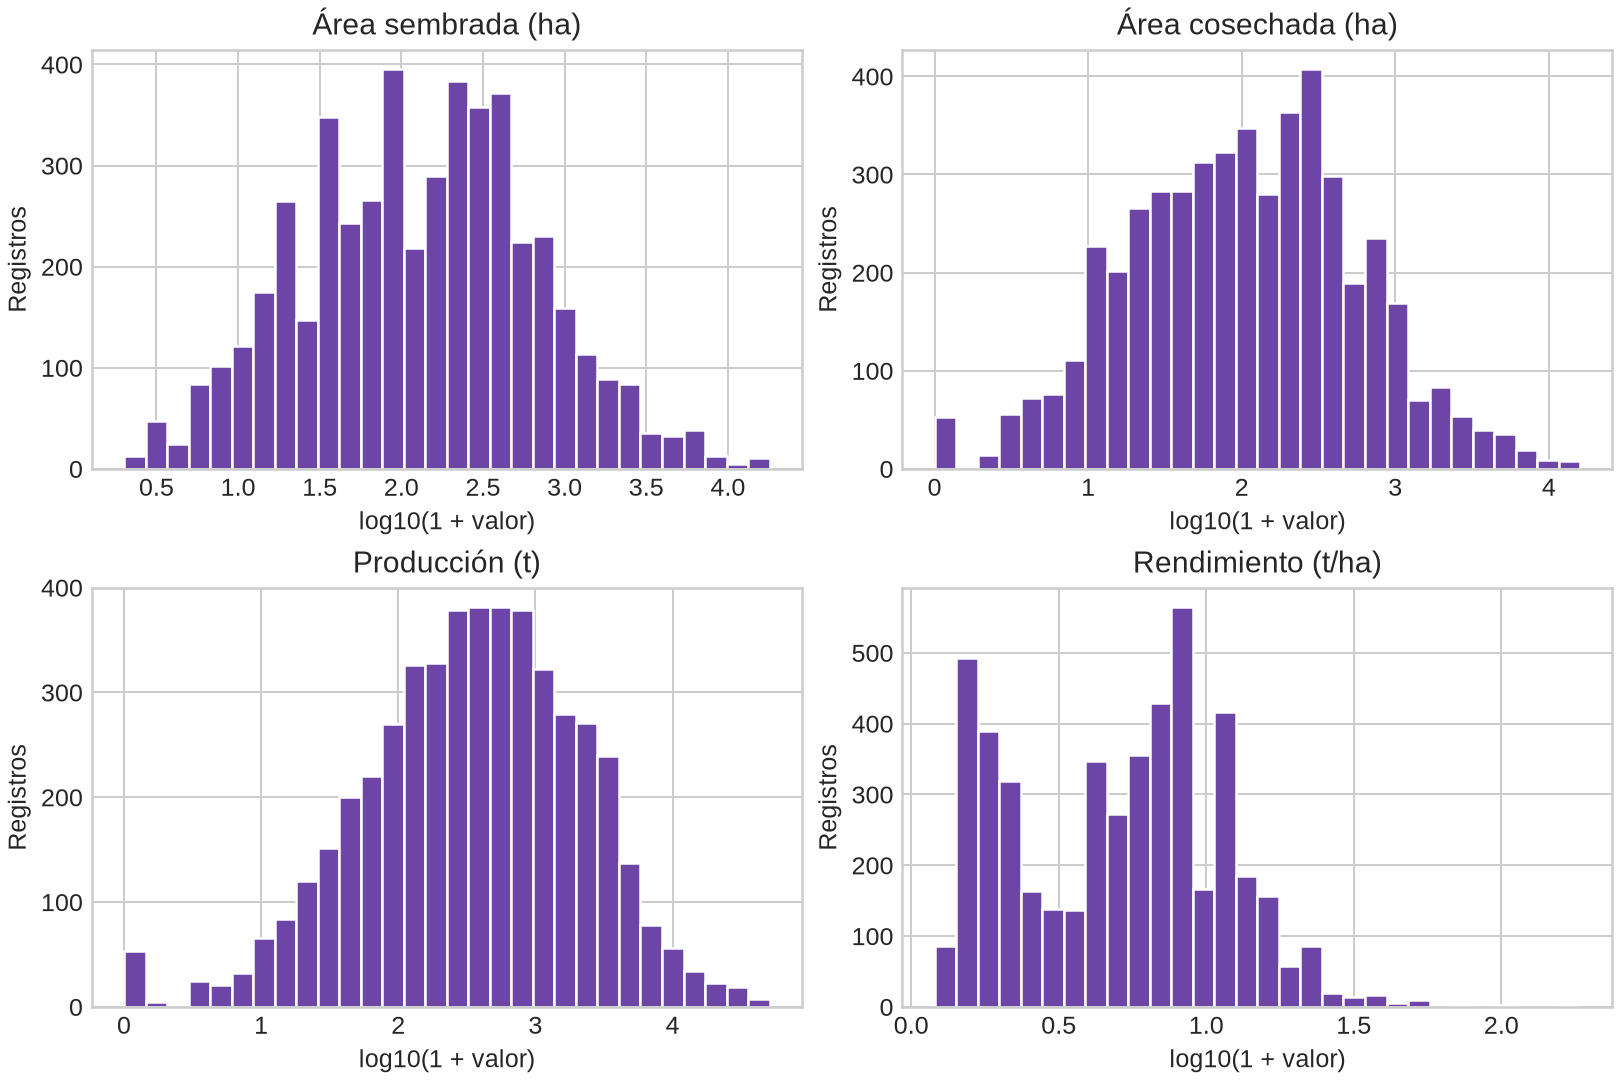
\includegraphics[width=\linewidth]{eva_Py_01_inspeccion.png}
\column{.39\textwidth}
\small
Cada barra cuenta registros en un intervalo.

\vspace{.5em}
El área sembrada llega a 18.000 ha.
Usamos \(u=\log_{10}(1+x)\) para mostrar juntas cantidades grandes y pequeñas.
El \(1+x\) permite incluir los ceros.
\end{columns}
\end{frame}

\begin{frame}{Mínimos, máximos y faltantes}
\small
4.887 registros del Cesar en 25 municipios, antes de limpiar y agrupar.
\vspace{.75em}

\centering
\begin{tabular}{lrrr}
\toprule
Variable & Mínimo & Máximo & Faltantes\\
\midrule
Área sembrada (ha) & 1 & 18.000 & 0\\
Área cosechada (ha) & 0 & 16.000 & 0\\
Producción (t) & 0 & 51.000 & 0\\
Rendimiento reportado (t/ha) & 0,20 & 184 & 53\\
\bottomrule
\end{tabular}

\vspace{.7em}
Los 53 rendimientos faltantes corresponden a registros sin cosecha.
Las demás columnas están completas.

\begin{block}{Pregunta del estudio}
¿Cómo se distribuye la variabilidad del rendimiento entre cultivos, municipios y años?
\end{block}
\end{frame}

\begin{frame}{Seis observaciones anuales fuera de las cercas del IQR}
\begin{columns}[c,totalwidth=\textwidth]
\column{.54\textwidth}
\centering
\scriptsize
\begin{tabular}{llrr}
\toprule
Cultivo & Municipio & Año & Rendimiento (t/ha)\\
\midrule
Café & Agustín Codazzi & 2011 & 0,20\\
Algodón & Chiriguaná & 2007 & 0,38\\
Arroz & Curumaní & 2016 & 1,44\\
Yuca & Río de Oro & 2016--2018 & 3,00 cada año\\
\bottomrule
\end{tabular}

\smallskip
2.123 rendimientos definidos. Al retirar seis, quedan 2.117.
\column{.43\textwidth}
\small
Por municipio, cultivo y año, sumamos la producción y el área cosechada.
En Curumaní, el arroz de 2016 da
\[
\frac{131+25}{88+20}=1{,}44\ \text{t/ha}.
\]
El IQR se calcula dentro de cada cultivo sobre \(\ln(Y)\).
Curumaní quedó por debajo de la cerca inferior del arroz, equivalente a 2,52 t/ha.
\end{columns}
\end{frame}

\begin{frame}{Rendimiento anual por cultivo}
\begin{columns}[c,totalwidth=\textwidth]
\column{.65\textwidth}
\centering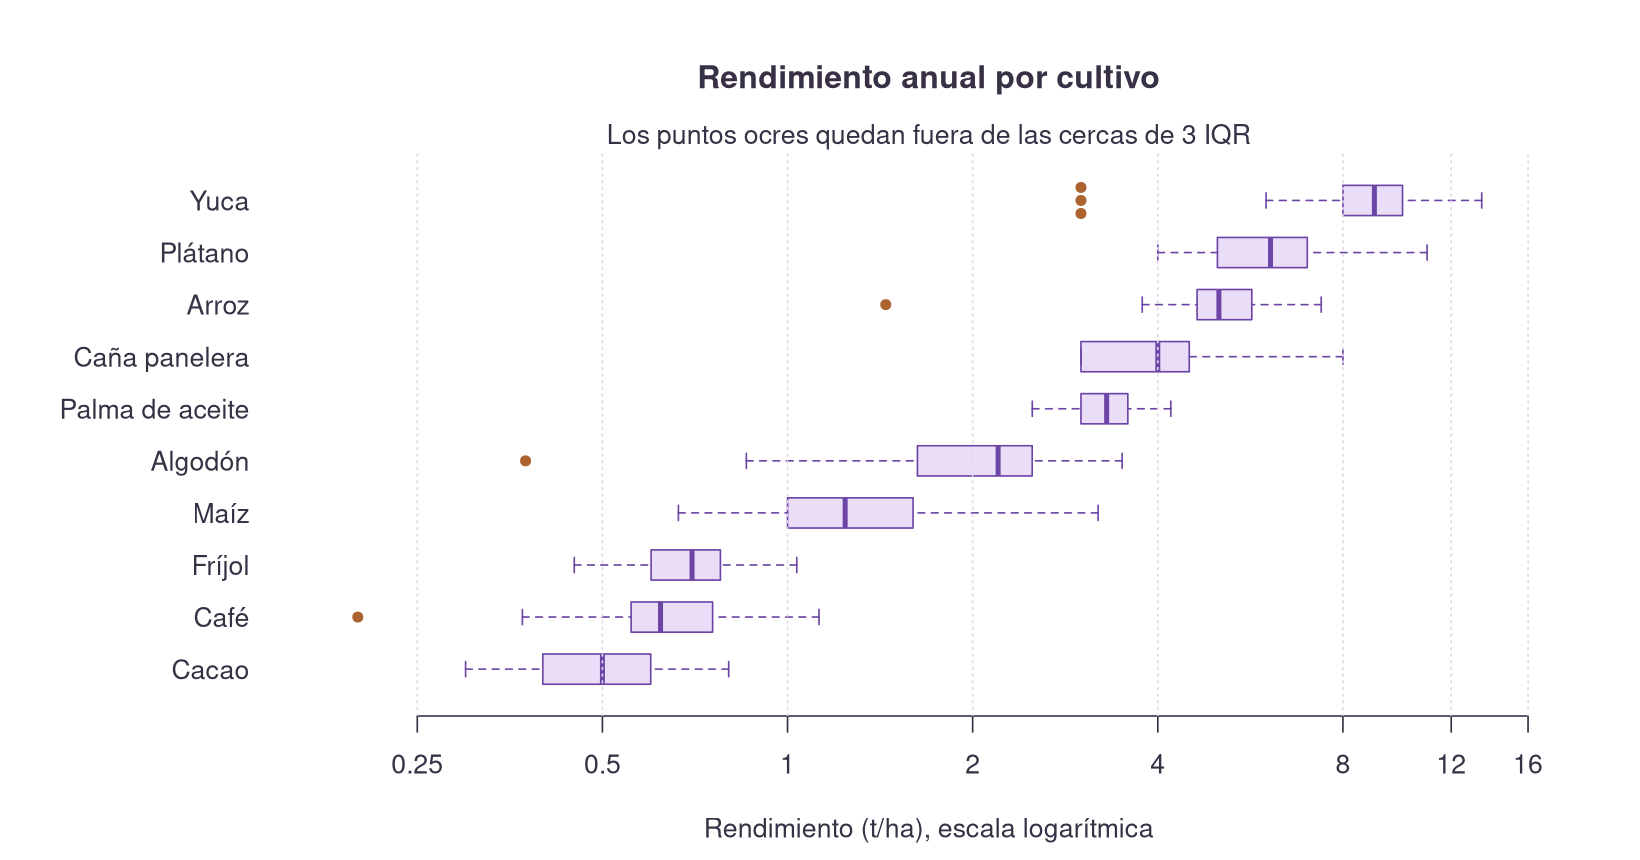
\includegraphics[width=\linewidth]{eva_R_02_cajas.png}
\column{.33\textwidth}
\small
La línea interior es la mediana. La caja reúne la mitad central y los puntos ocres
marcan los seis extremos.

\smallskip
Los tres puntos de yuca coinciden en 3,00 t/ha y se separan verticalmente.
El eje muestra t/ha en escala logarítmica.
\end{columns}
\end{frame}

\begin{frame}{Mediana y dispersión en la base depurada}
\begin{columns}[c,totalwidth=\textwidth]
\column{.62\textwidth}
\centering\scriptsize
\begin{tabular}{lrrrrr}
\toprule
Cultivo & \(n\) & \(Q_1\) & Mediana & \(Q_3\) & DE\\
\midrule
Algodón & 92 & 1,64 & 2,20 & 2,50 & 0,67\\
Arroz & 215 & 4,64 & 5,03 & 5,69 & 0,79\\
Cacao & 219 & 0,40 & 0,50 & 0,60 & 0,11\\
Café & 227 & 0,56 & 0,62 & 0,76 & 0,16\\
Caña panelera & 89 & 3,00 & 4,00 & 4,50 & 1,05\\
Fríjol & 224 & 0,60 & 0,70 & 0,78 & 0,14\\
Maíz & 289 & 1,00 & 1,24 & 1,60 & 0,60\\
Palma de aceite & 241 & 3,00 & 3,30 & 3,58 & 0,51\\
Plátano & 236 & 5,00 & 6,10 & 7,00 & 1,65\\
Yuca & 285 & 8,00 & 9,03 & 10,00 & 1,81\\
\bottomrule
\end{tabular}
\column{.35\textwidth}
\small
\(n\) cuenta combinaciones de municipio y año. La yuca tiene mediana de 9,03 t/ha
y el cacao de 0,50 t/ha.

\smallskip
\(Q_1\) y \(Q_3\) delimitan la mitad central. DE es la desviación estándar, en t/ha.
\end{columns}
\end{frame}

\begin{frame}{El 90,59\,\% de la variabilidad separa a los cultivos}
\begin{columns}[c,totalwidth=\textwidth]
\column{.68\textwidth}
\centering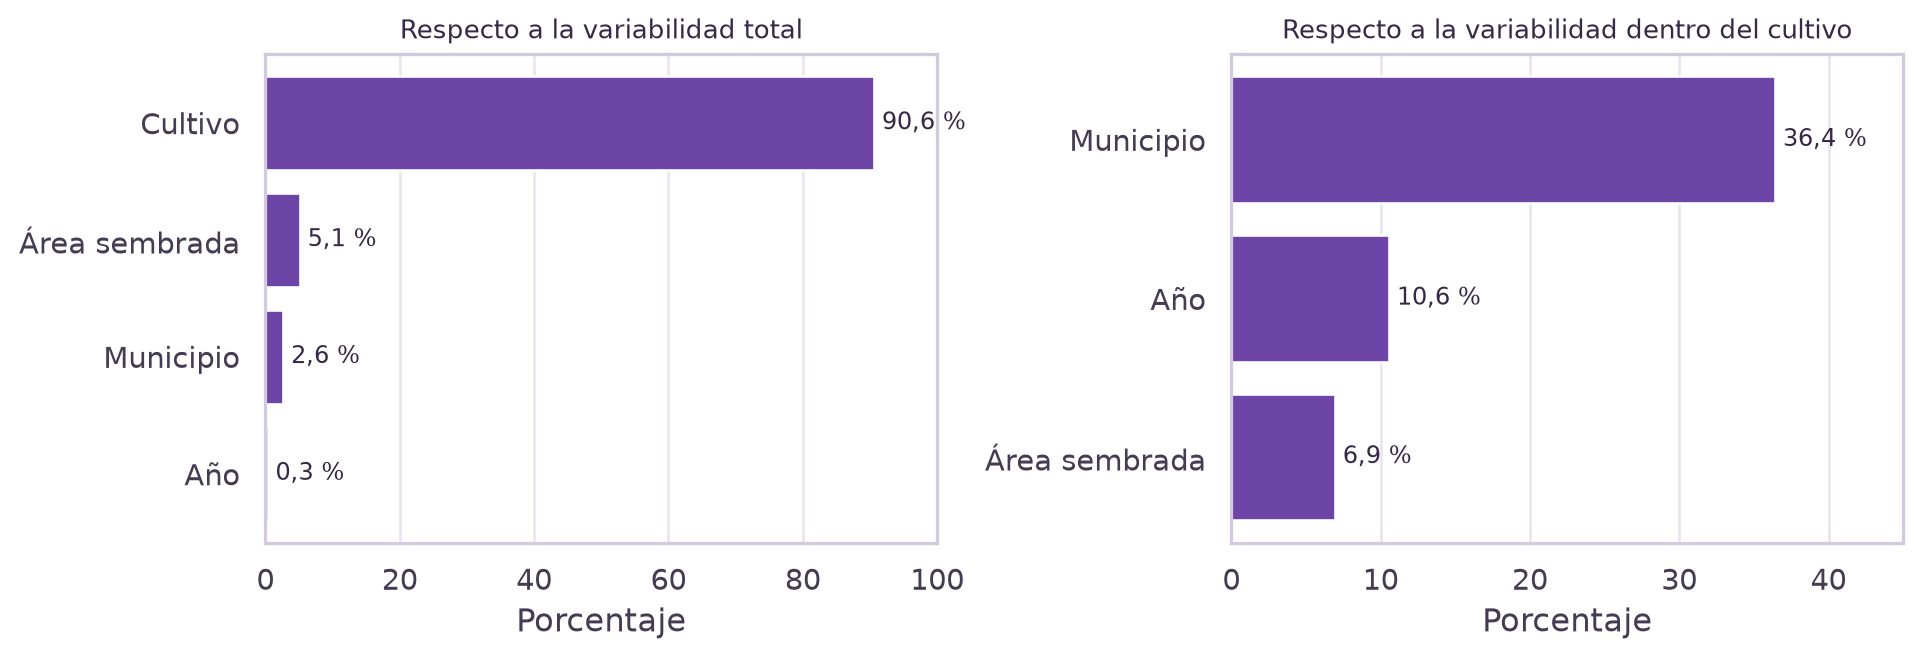
\includegraphics[width=\linewidth]{eva_Py_10_variabilidad.png}
\column{.30\textwidth}
\small
Usamos \(n_c\) registros, media \(\bar y_c\) por cultivo y media general \(\bar y\).
\[
\frac{\sum_c n_c(\bar y_c-\bar y)^2}
     {\sum_i(y_i-\bar y)^2}
=0{,}9059.
\]
Dentro del mismo cultivo, el municipio reúne la mayor fracción en t/ha (36,42\,\%).
Las fracciones de municipio, año y área pueden solaparse.
\end{columns}
\end{frame}

\begin{frame}{Cobertura municipal por cultivo y año}
\begin{columns}[c,totalwidth=\textwidth]
\column{.67\textwidth}
\centering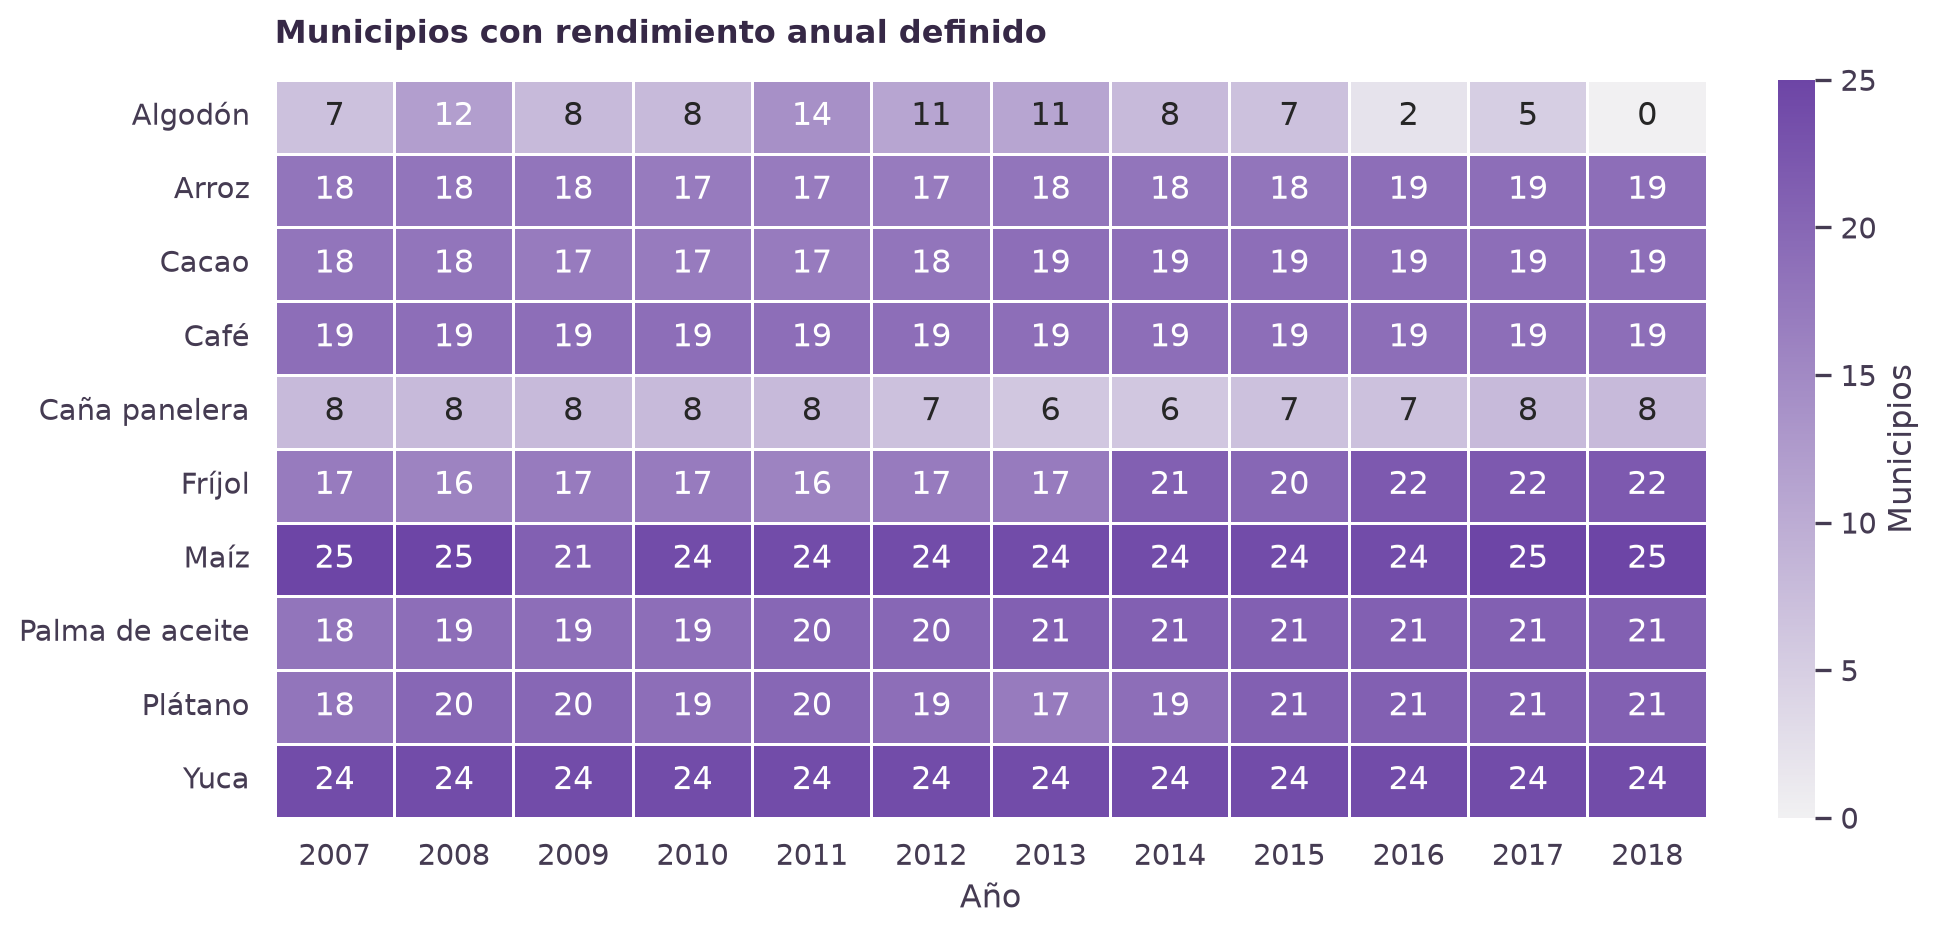
\includegraphics[width=\linewidth]{eva_Py_06_cobertura.png}
\column{.30\textwidth}
\small
Cada celda cuenta municipios con rendimiento definido.

\smallskip
La yuca tiene 24 cada año. Para algodón, el número pasa de 14 en 2011 a dos en 2016
y a cero en 2018.
\end{columns}
\end{frame}

\begin{frame}{Trayectoria anual del rendimiento departamental}
\begin{columns}[c,totalwidth=\textwidth]
\column{.65\textwidth}
\centering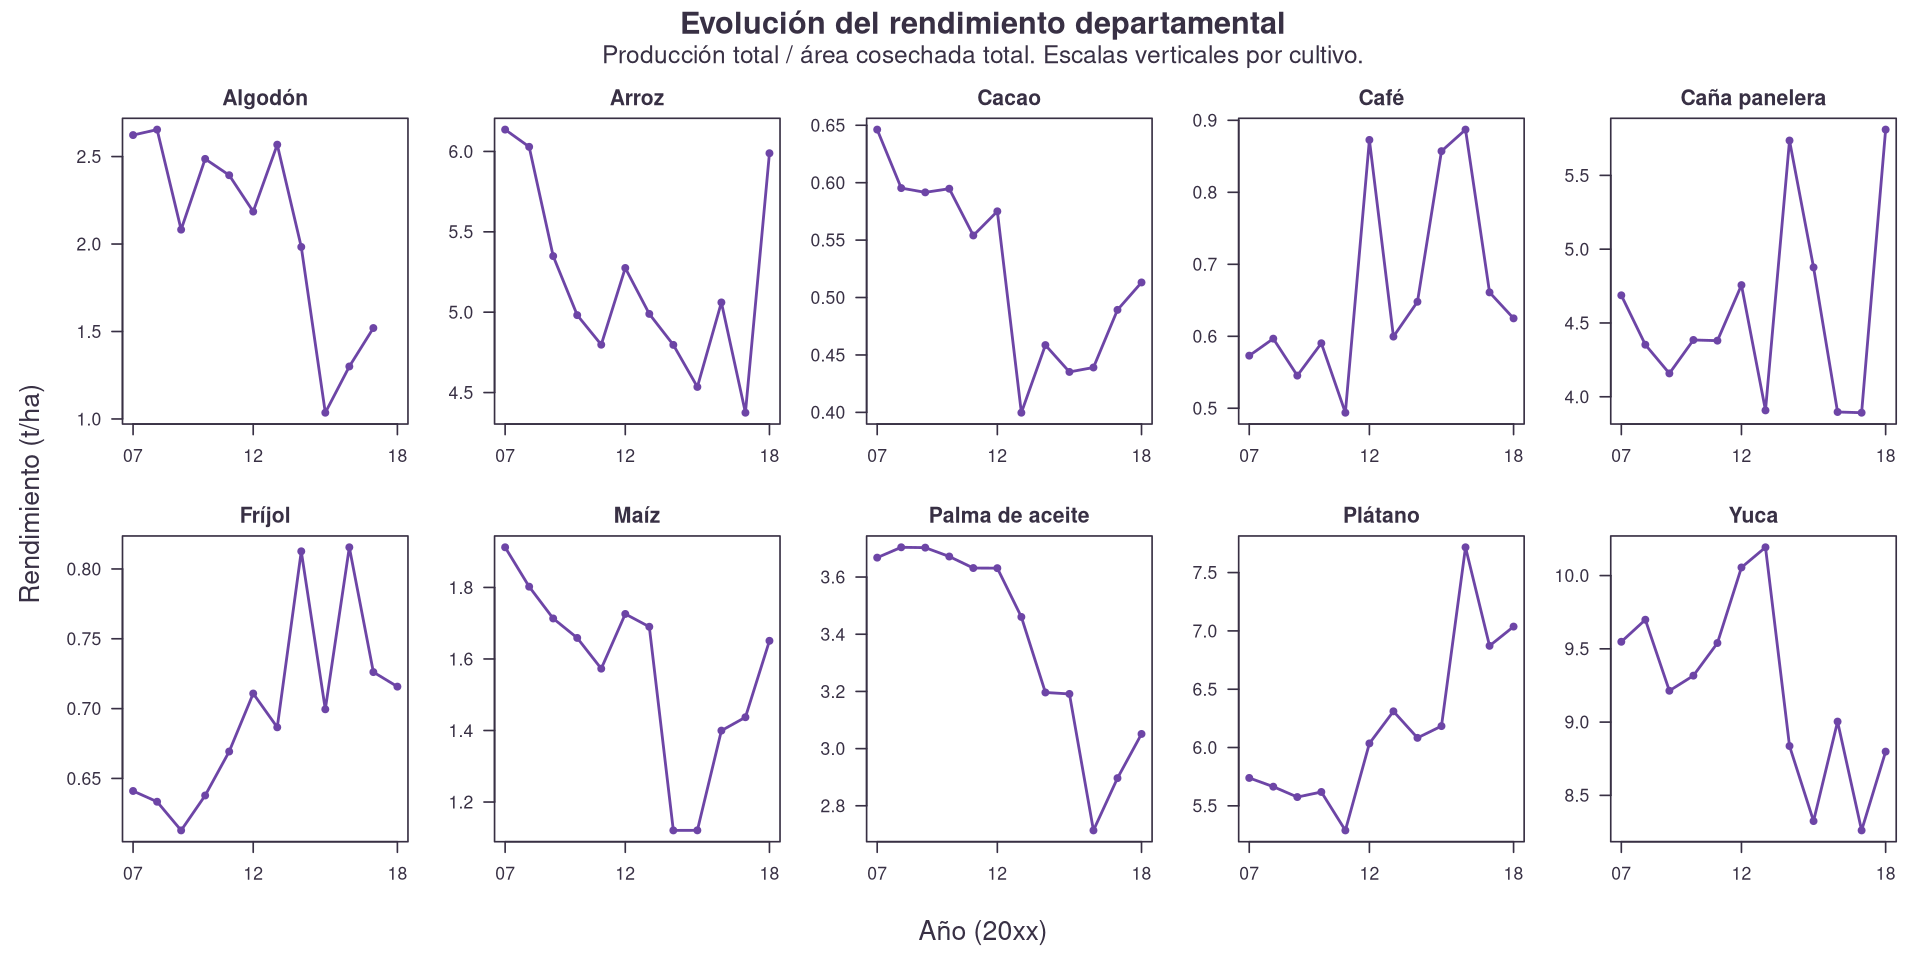
\includegraphics[width=\linewidth]{eva_R_04_trayectorias.png}
\column{.33\textwidth}
\small
Cada punto divide la producción total por el área cosechada total del cultivo en el año.

\smallskip
En arroz, el punto de 2018 es \(46\,247/7\,722=5{,}99\) t/ha. Cada panel usa su propia escala vertical.
\end{columns}
\end{frame}

\begin{frame}{Las diferencias territoriales dependen del cultivo}
\begin{columns}[c,totalwidth=\textwidth]
\column{.55\textwidth}
\centering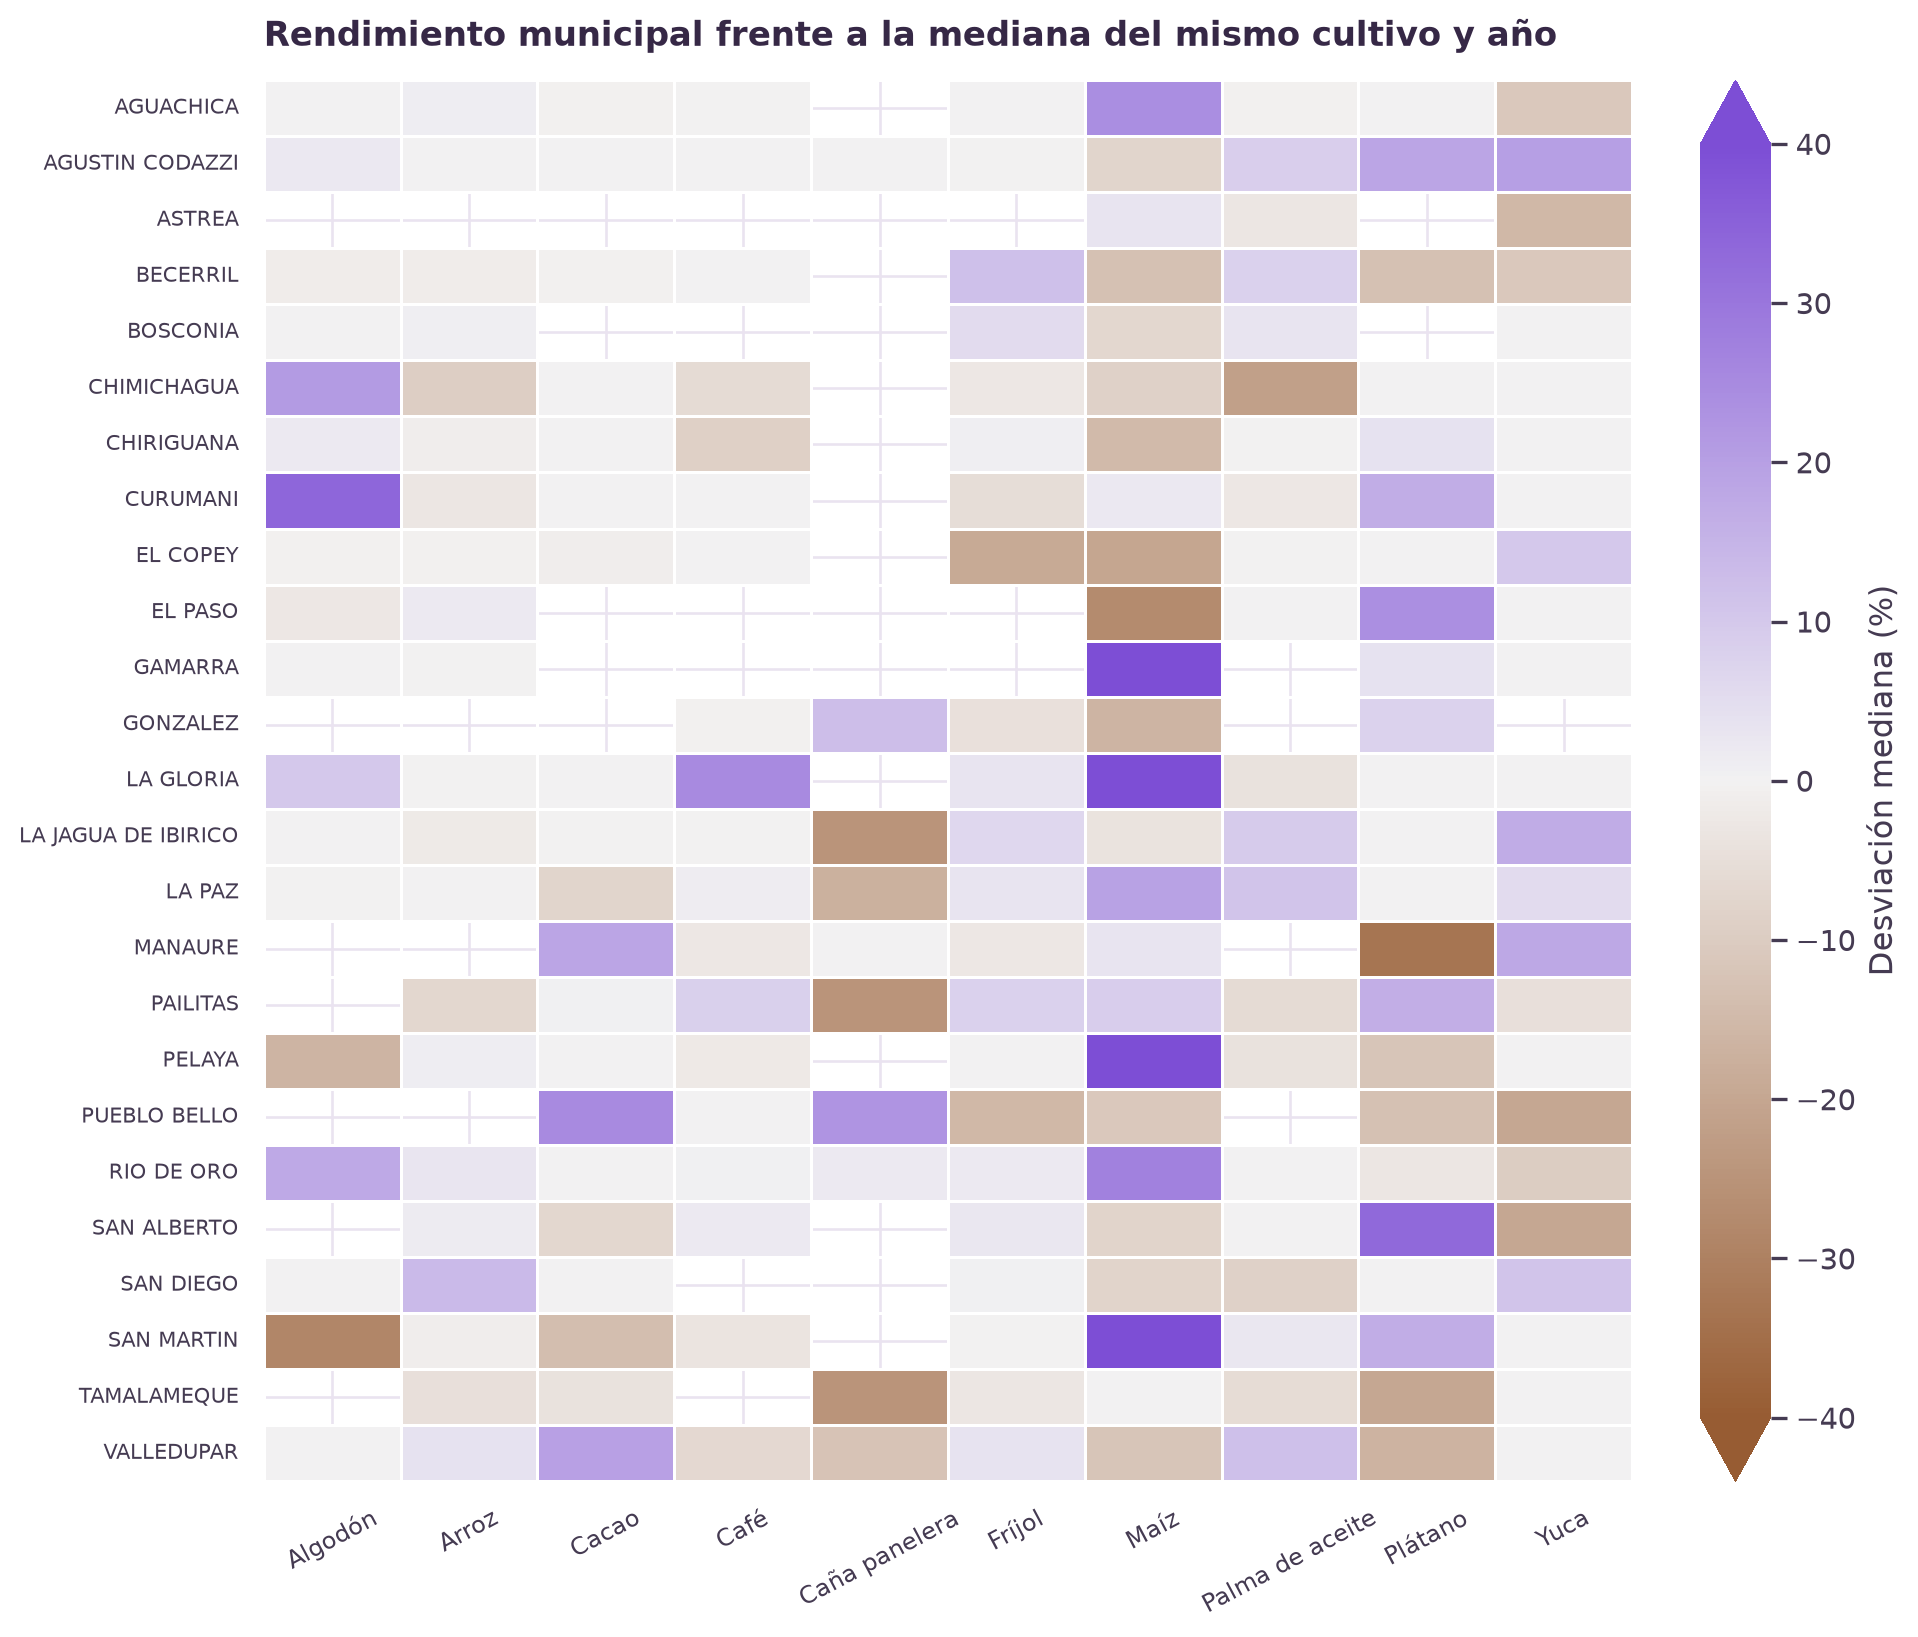
\includegraphics[height=.70\textheight]{eva_Py_07_territorio.png}
\column{.43\textwidth}
Comparamos cada municipio con la mediana del mismo cultivo y año.
\vspace{.6em}

Los dos municipios tienen 12 años de maíz observados.
\begin{itemize}
\item San Martín queda 1,82 t/ha por encima de la referencia mediana.
\item El Paso queda 0,31 t/ha por debajo.
\end{itemize}
\end{columns}
\end{frame}

\begin{frame}{Conclusiones}
\begin{itemize}
\item Las diferencias entre cultivos reúnen el 90,59\,\% de la variabilidad en t/ha.
Al incluir los seis extremos, la fracción es 89,97\,\%.
\item Dentro de los cultivos, el municipio reúne la mayor fracción (36,42\,\%).
El año reúne el 10,56\,\% y los grupos de área sembrada, el 6,93\,\%.
Las tres fracciones pueden solaparse.
\item La cobertura influye en la lectura de las trayectorias.
La yuca tiene 24 municipios con datos cada año. El algodón carece de datos en 2018.
\end{itemize}
\end{frame}
\end{document}
